\documentclass[10pt]{beamer}
\usepackage{graphicx}
\usepackage{multicol}

\title{A5 Group CAD \\Project Gemini}
\author{Ahmed Woodson, Mark DeVince, Charles Hanner, Blaire Weinberg, Hyunsoo Chun}
\date{\today}

\graphicspath{{./Images/}}


\begin{document}
	\frame{\titlepage}
	
\section{Group}
	
	\begin{frame}{Group Beauty Shot}
		\begin{minipage}{0.49\textwidth}
			\begin{itemize}
				\item Gemini was a 2 crew Apollo proving ground
				\item Launch mass was 3.8 MT, with 455 kg of propellant
				\item 12 Gemini flights were flown, with duration between 5 hours and 14 days
			\end{itemize}
		\end{minipage}%
		\begin{minipage}{0.49\textwidth}
			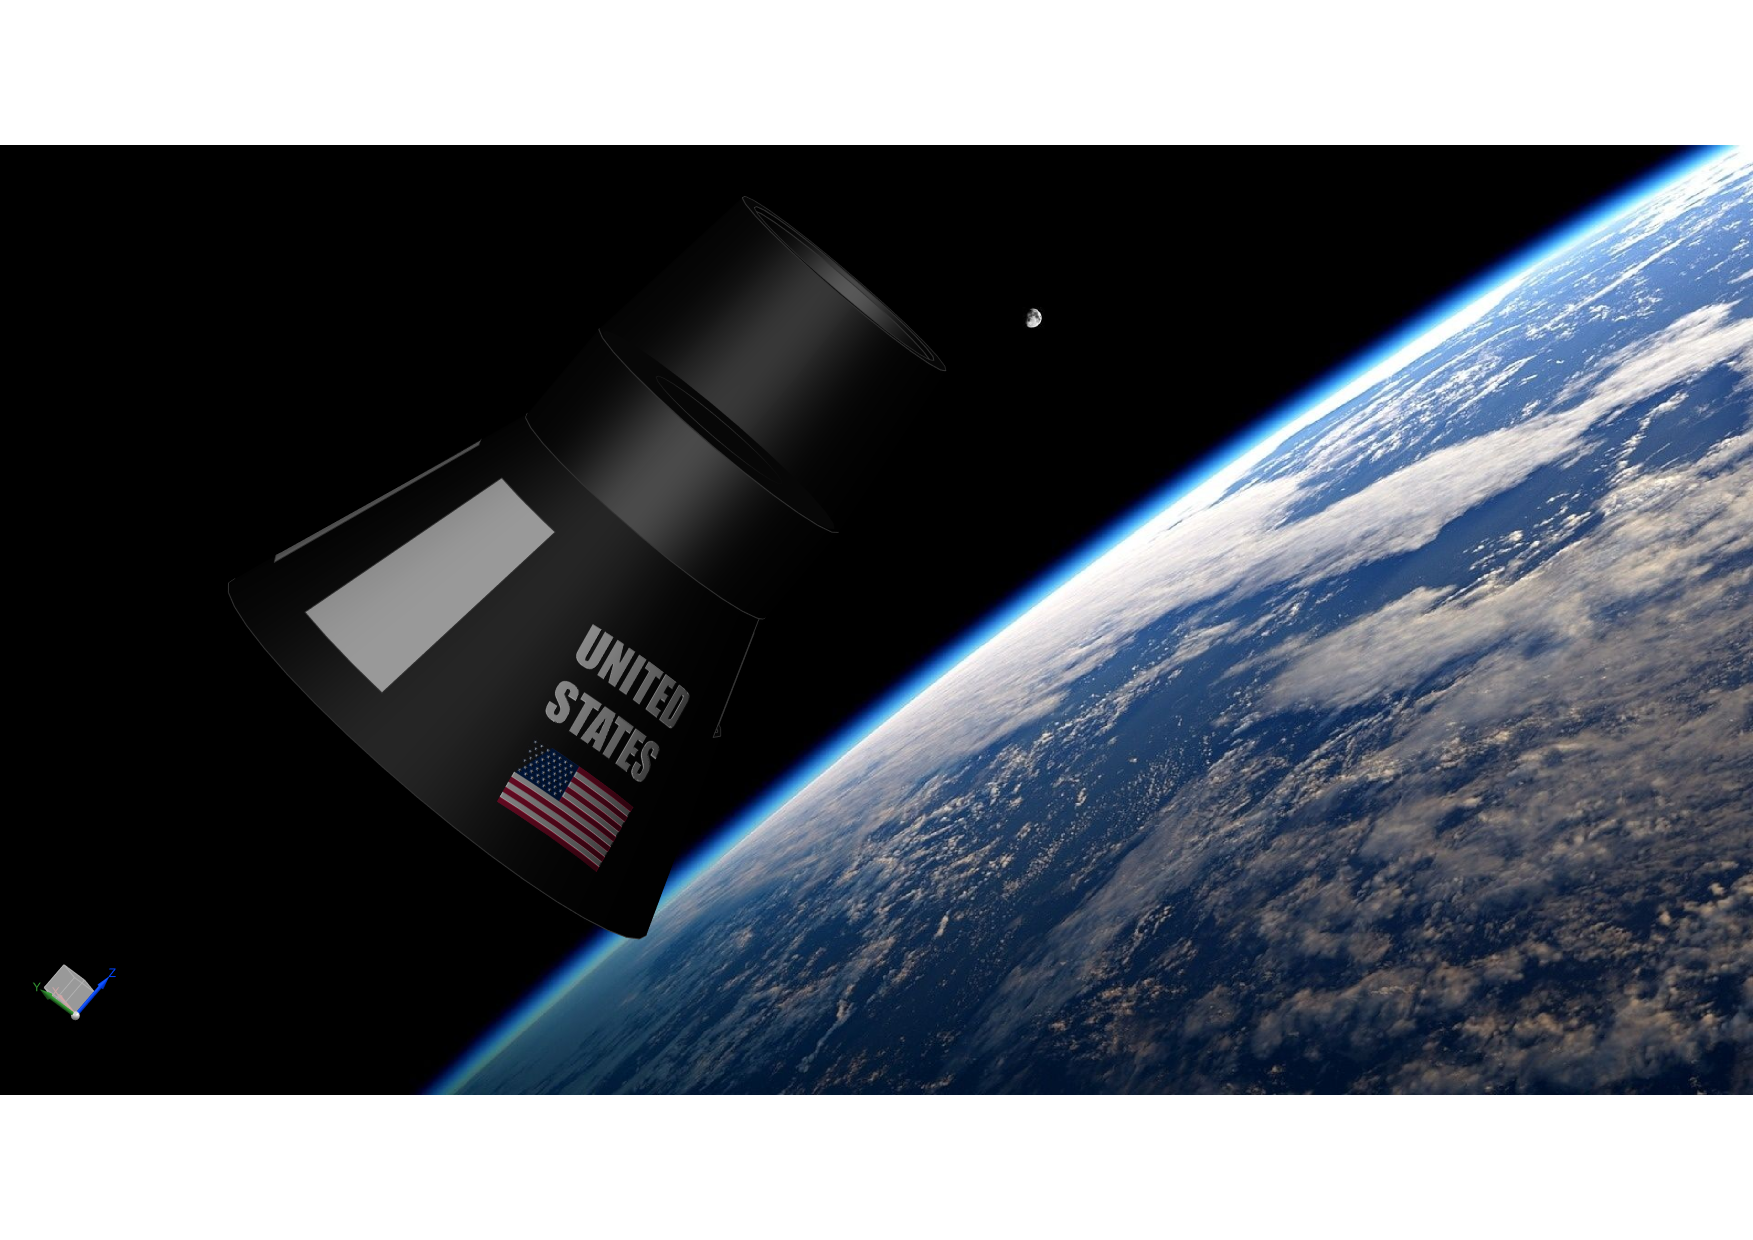
\includegraphics[width=\textwidth]{Group_Beauty.png}
		\end{minipage}
	\end{frame}

	\begin{frame}{External 3 View}
		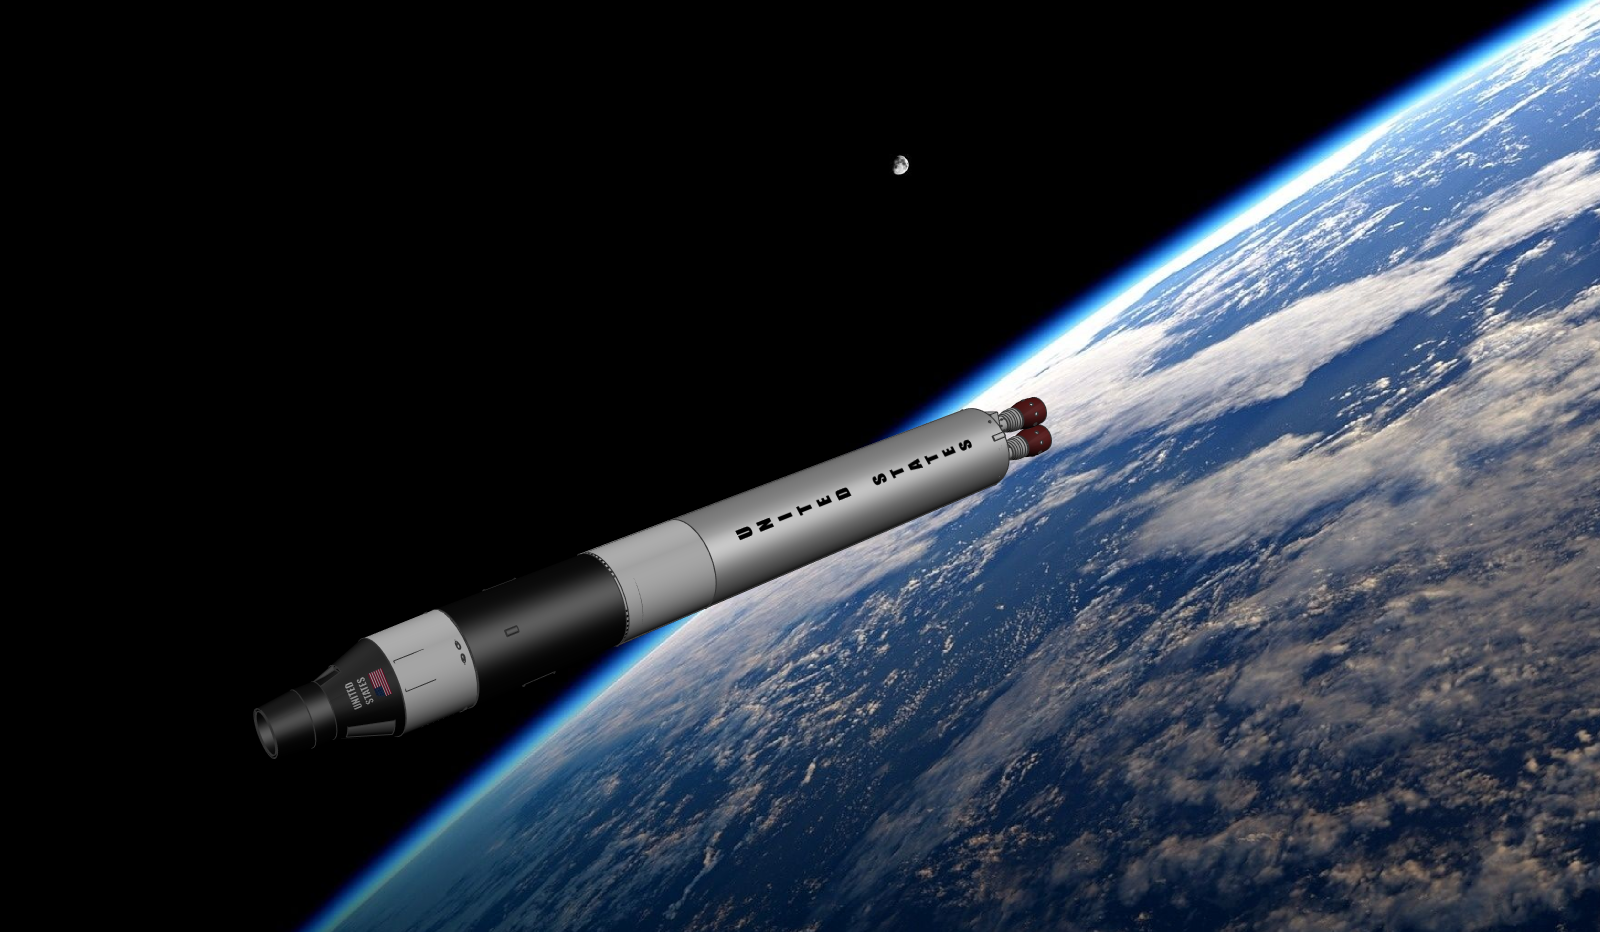
\includegraphics[width=\textwidth]{External_3_View.png}
	\end{frame}

	\begin{frame}{Interior View}
		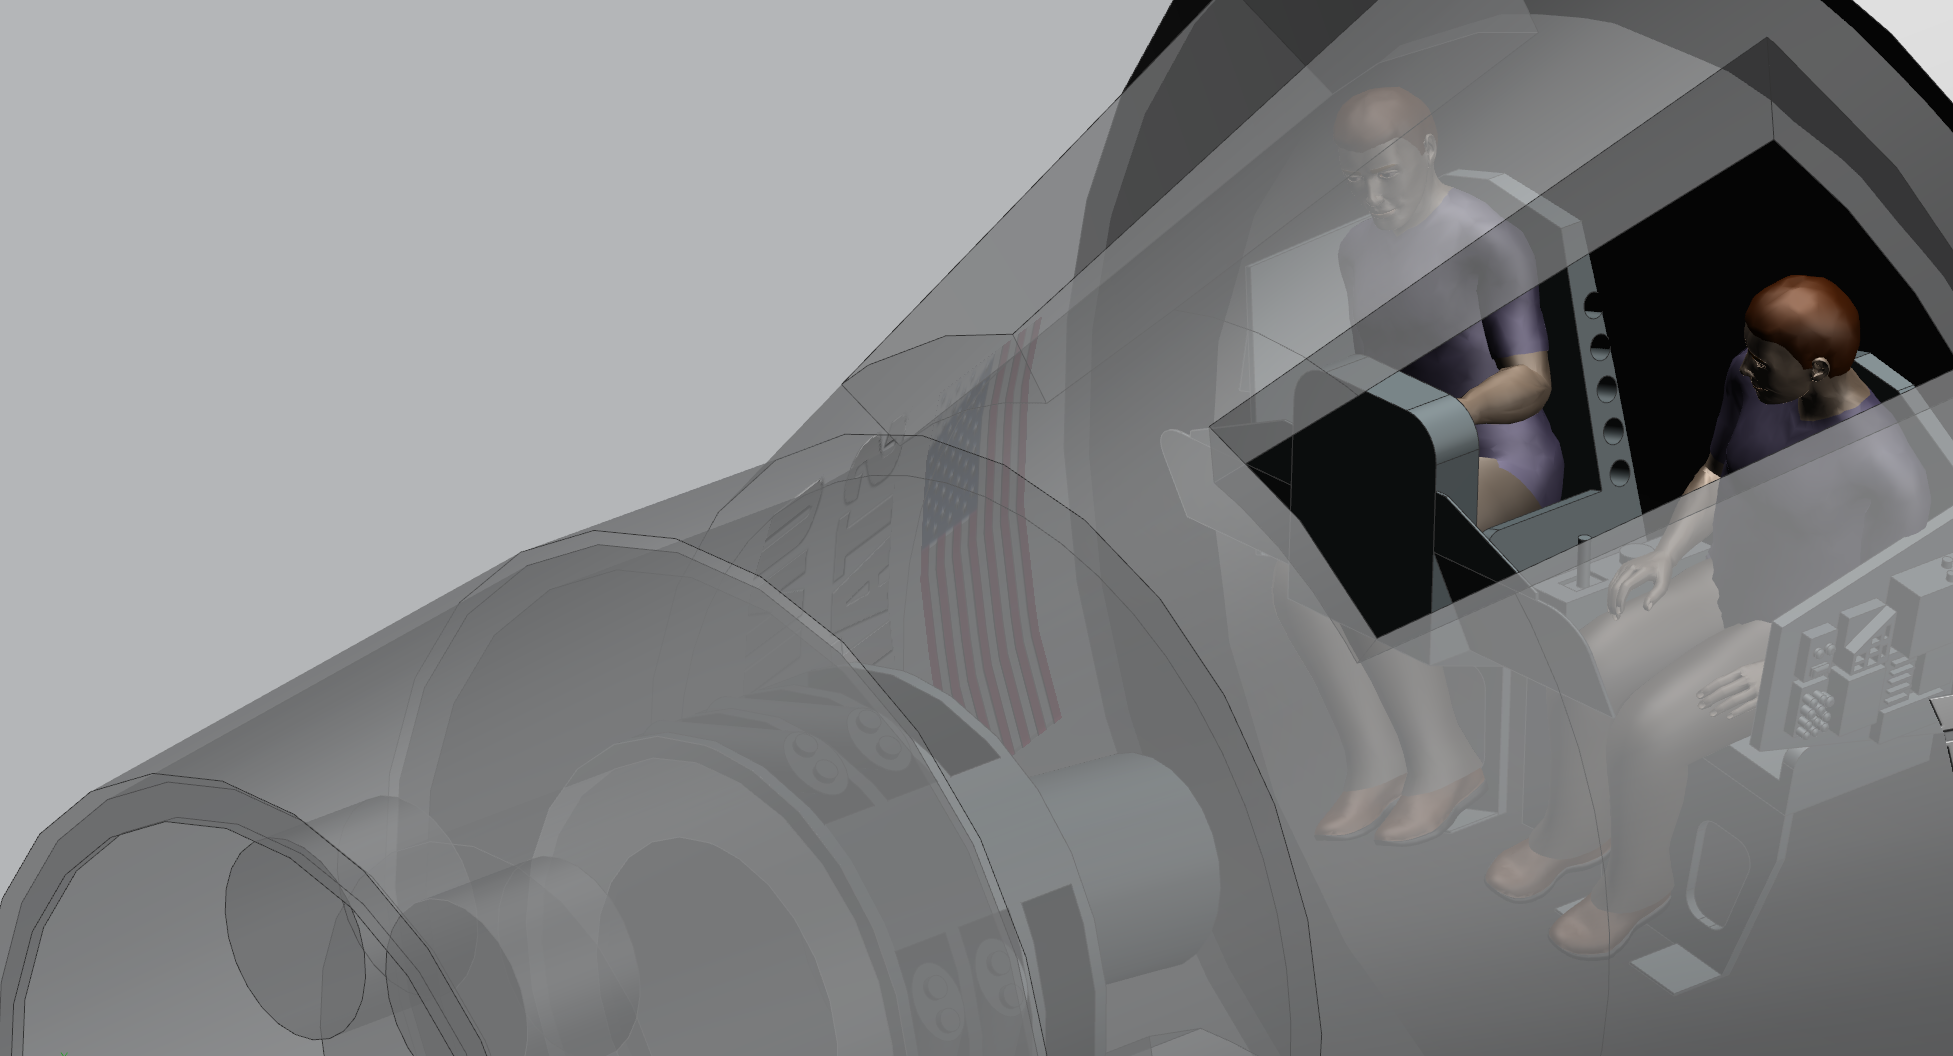
\includegraphics[width=\textwidth]{Interior_View.png}
	\end{frame}

	\begin{frame}{Color Coded}
		\begin{minipage}{0.45\textwidth}
			\begin{table}
				\begin{tabular}{|c|c|}\hline
					\textbf{Person} & \textbf{Color}\\ \hline
					Ahmed Woodson & Blue\\ \hline
					Mark DeVince & Magenta\\  \hline
					Charles Hanner & Green\\ \hline
					Blaire Weinberg & Grey\\  \hline
					Hyunsoo Chun & Red\\ \hline
				\end{tabular}
			\end{table}	
		
		For a full list of parts, please\\ see the last slide
		\end{minipage}%
		\begin{minipage}{0.54\textwidth}
			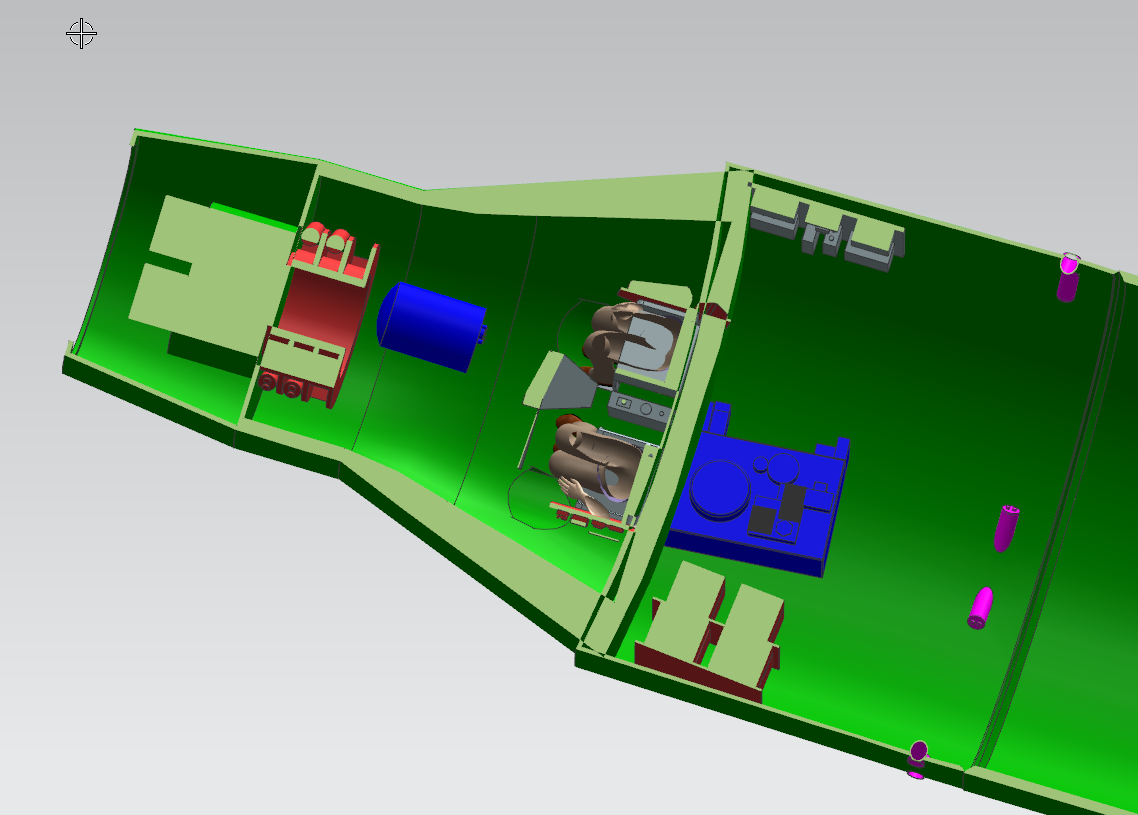
\includegraphics[width=\textwidth]{Color_Coded_Interior.png}			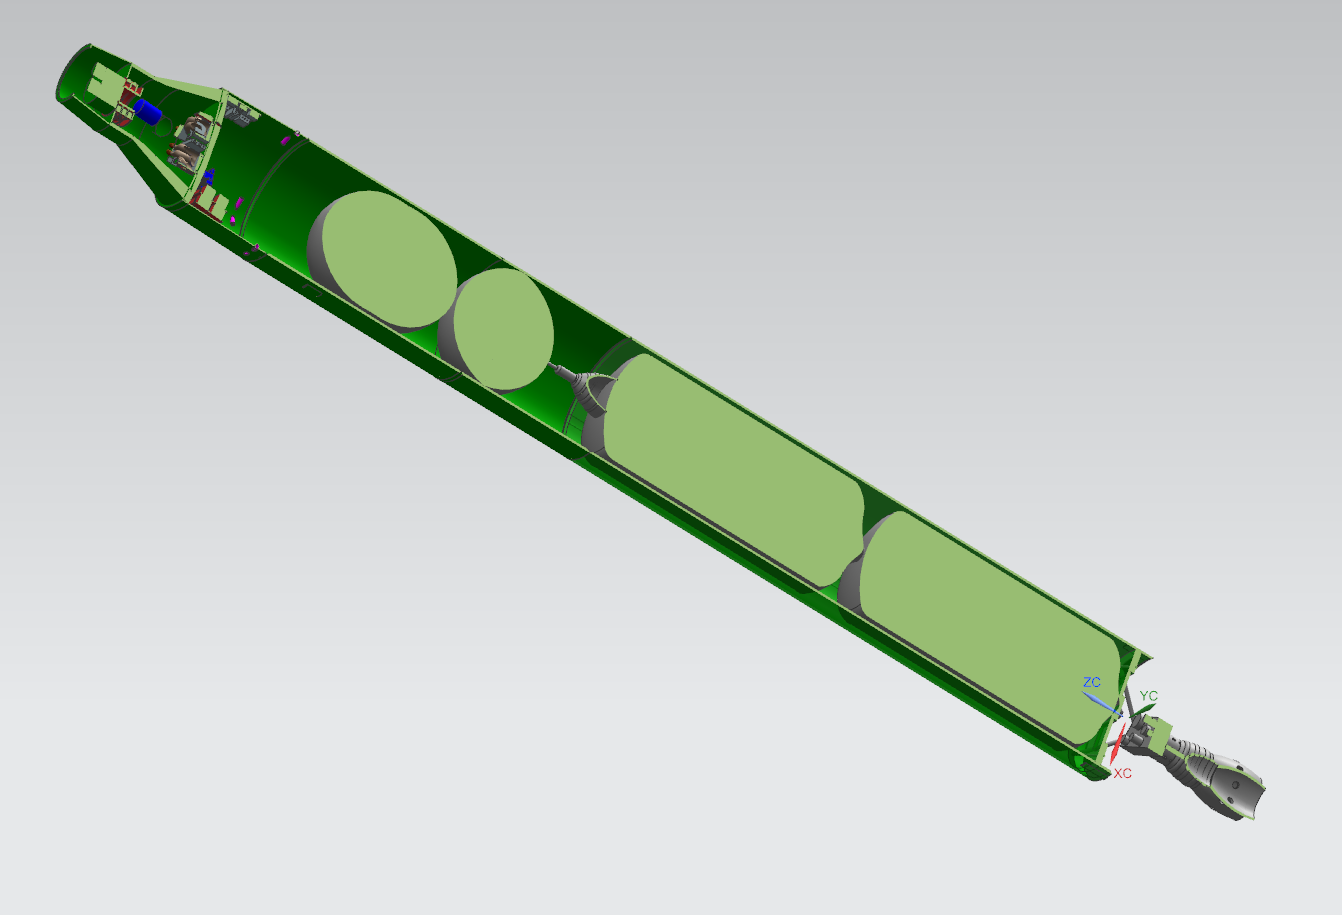
\includegraphics[width=\textwidth]{Color_Coded_Full.png}
		\end{minipage}
	\end{frame}
	\begin{frame}{Launch Vehicle}
		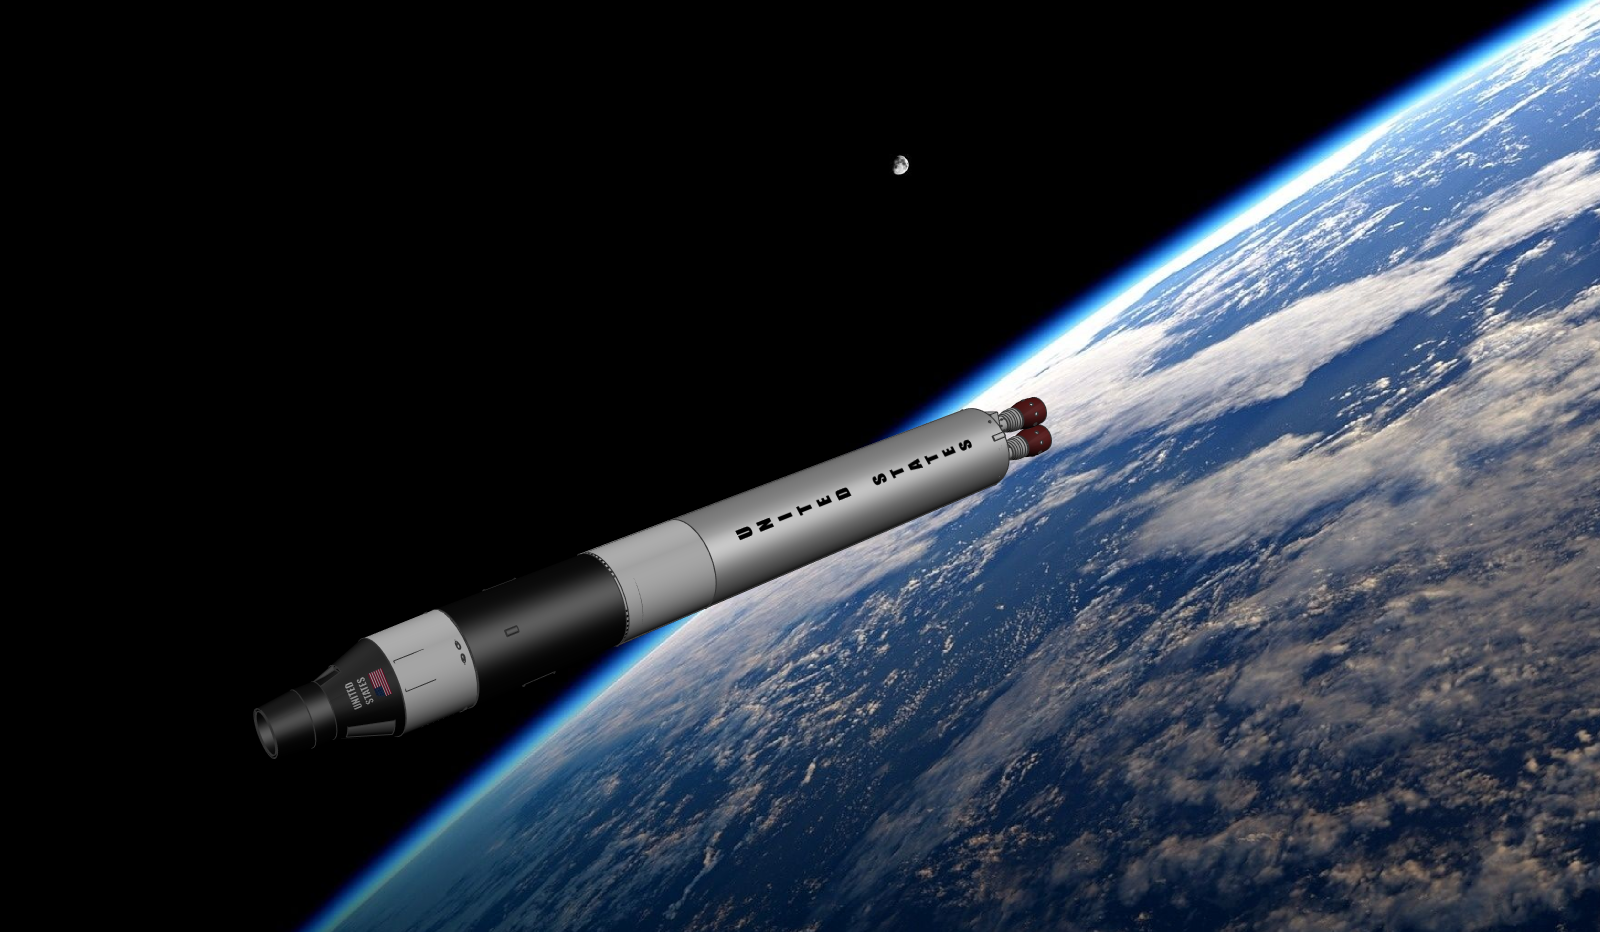
\includegraphics[width=\textwidth]{Launch_Vehicle.png}
	\end{frame}

	\begin{frame}{Baseball Card}
		\begin{minipage}{0.48\textwidth}
\begin{figure}[H]
	\centering
	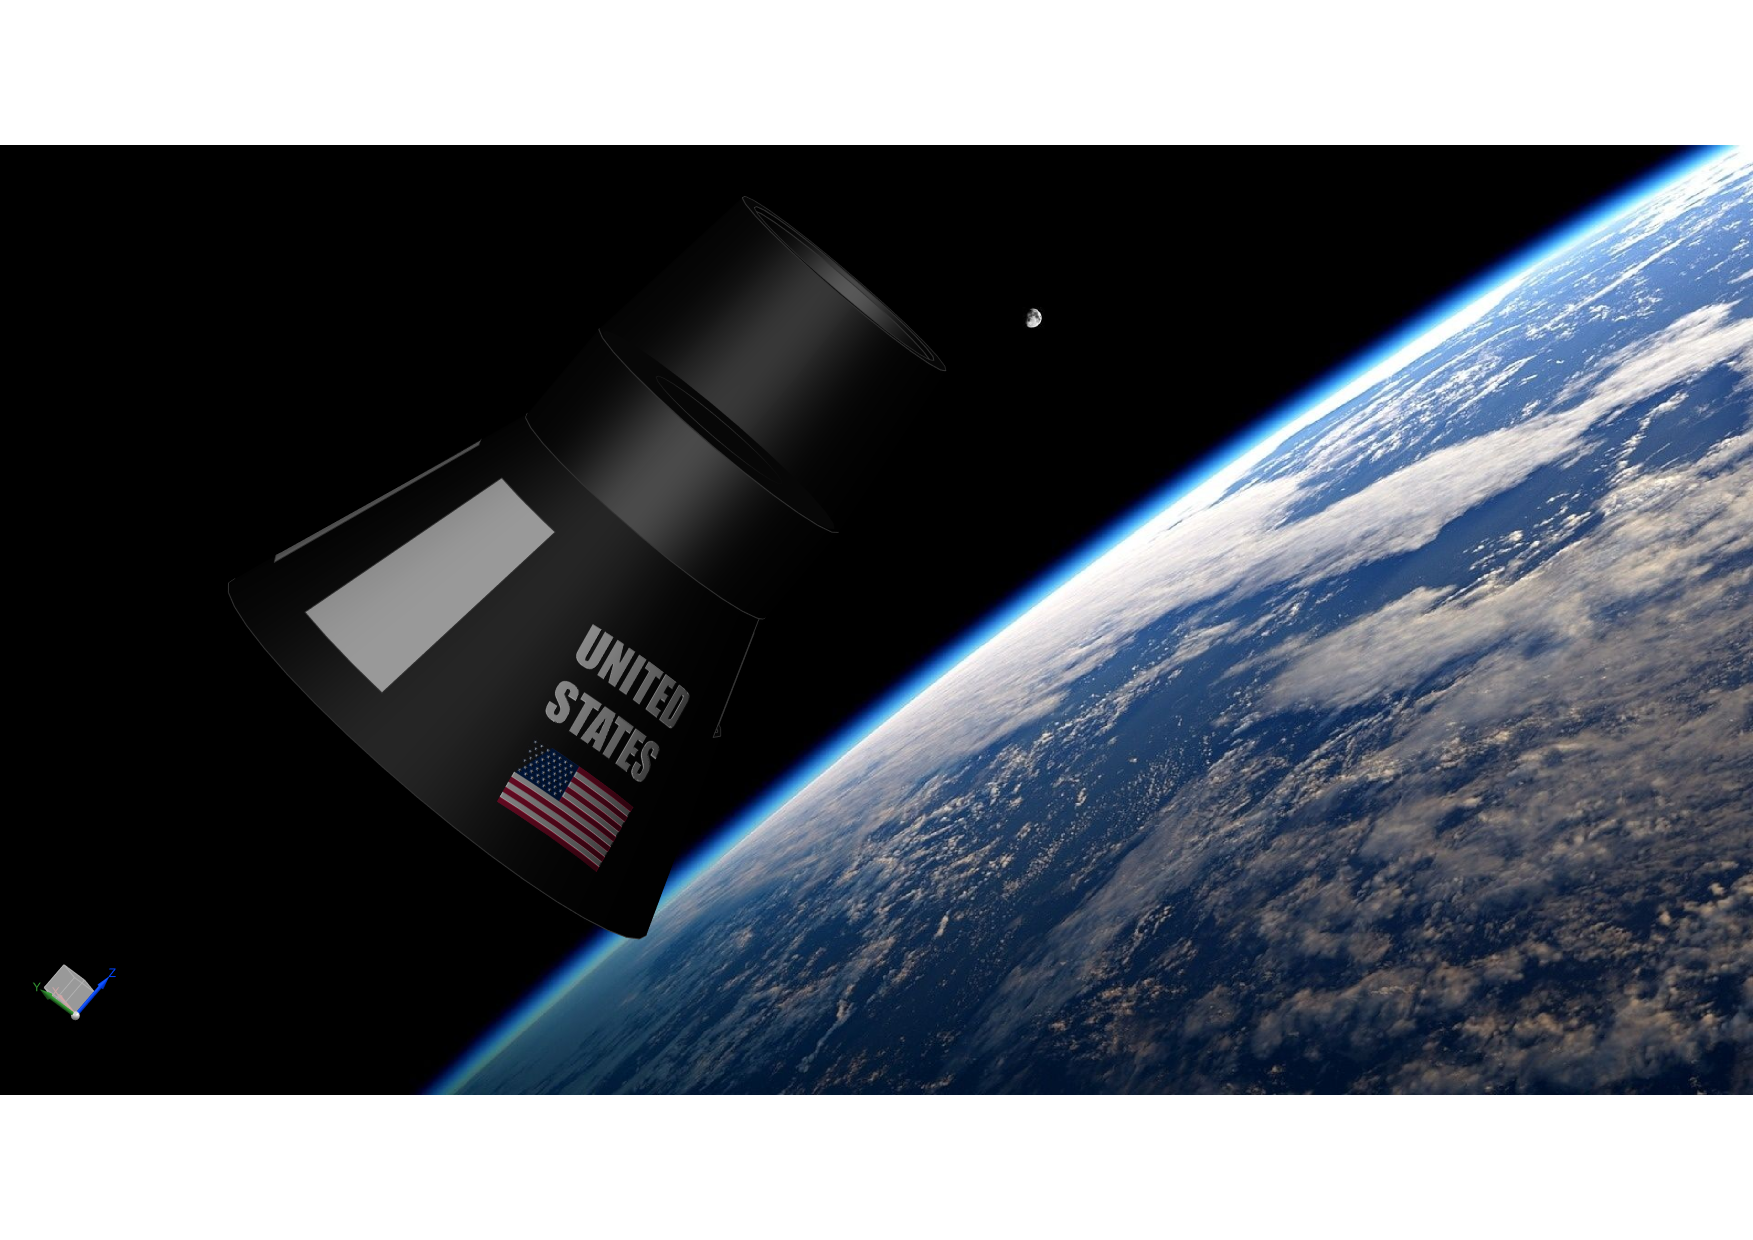
\includegraphics[width=\textwidth]{CapsuleOpaque.png}
\end{figure}
\tiny{The Gemini Program hosted by NASA between 1961 and 1967 had an estimated value of 1.3 \$B (7.6 \$B in 2018 value) and launched a total of twelve missions, of which ten were manned missions. Gemini was a precursor test program for the rapidly developing Apollo mission, and allowed Michael Collins (Gemini 10), Buzz Aldrin (Gemini 12), and Neil Armstrong (Gemini 8) to get to the moon. Additionally Pete Conrad (Gemini 5, 11), David Scott (Gemini 8), John Young (Gemini 3, 12), and Eugene Cernan (Gemini 9A) were also Apollo astronauts selected from this program. Gemini longstanding is viewed as a testbed and foundational program for modern spaceflight by experimenting with docking and EVAs. }


	\end{minipage}%
\begin{minipage}{0.49\textwidth}
	\begin{figure}
		\centering
		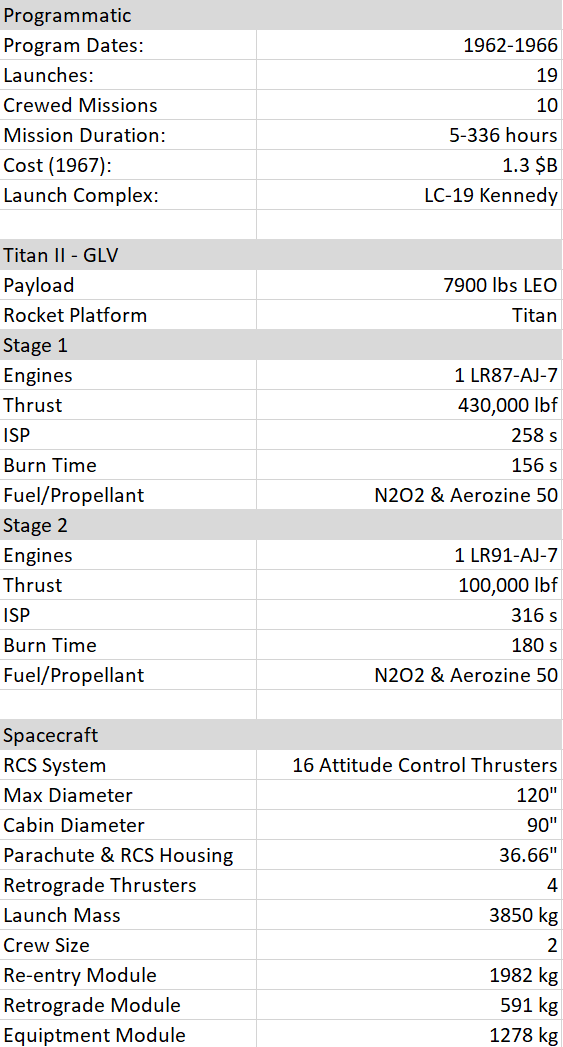
\includegraphics[width=0.8\textwidth]{baseball.png}
	\end{figure}
	
\end{minipage}

\end{frame}

\begin{frame}{Mission Profile}
	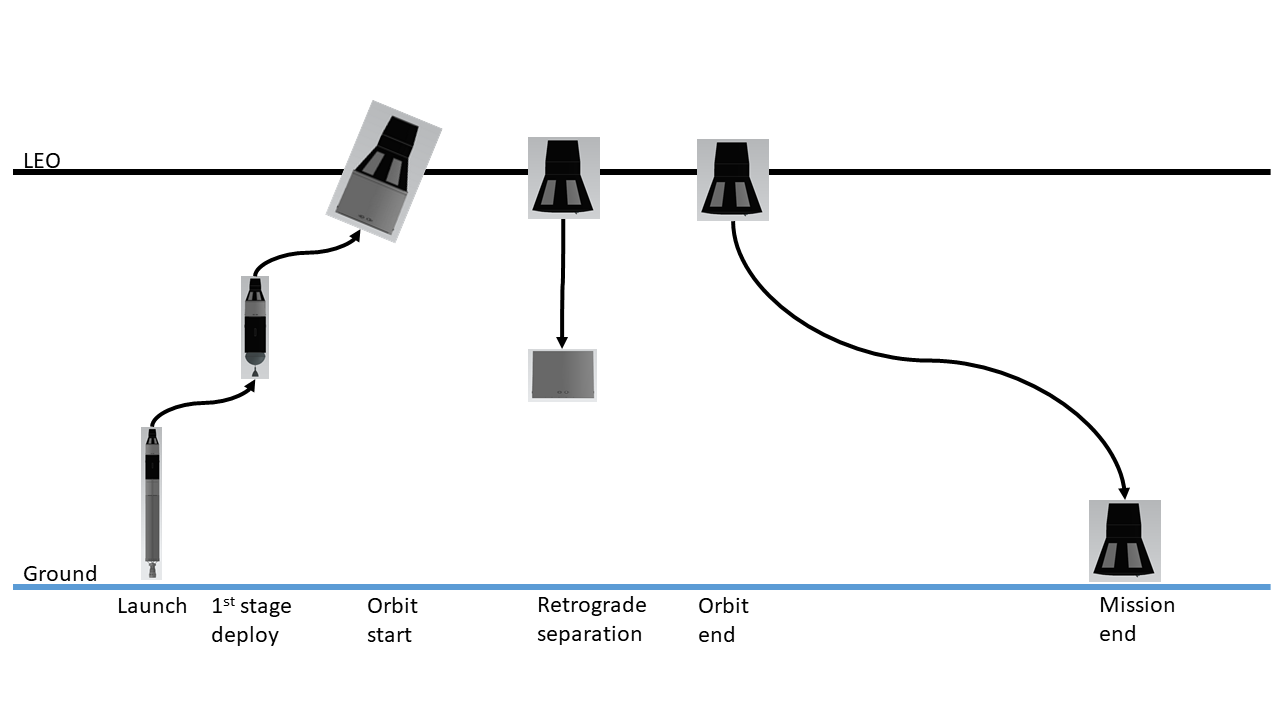
\includegraphics[width=\textwidth]{mission_profile.png}
\end{frame}


\section{individual}


	\begin{frame}{Woodson: Beauty Shot}
\begin{figure}
	\centering
	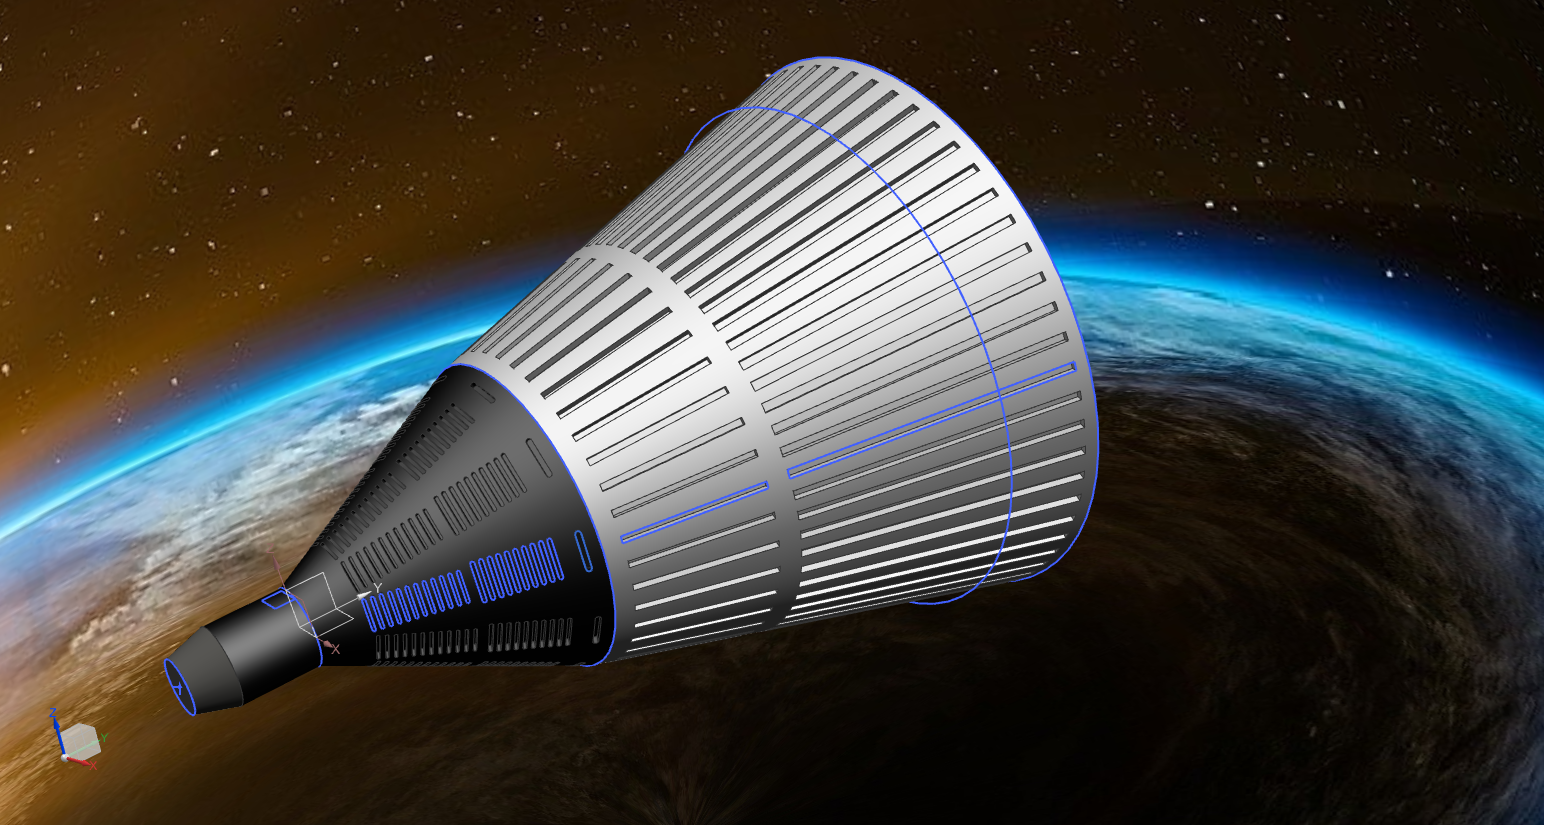
\includegraphics[width=\textwidth]{Woodson_Beauty.png}
\end{figure}
\end{frame}

	\begin{frame}{Woodson: 3 View}
\begin{figure}
	\centering
	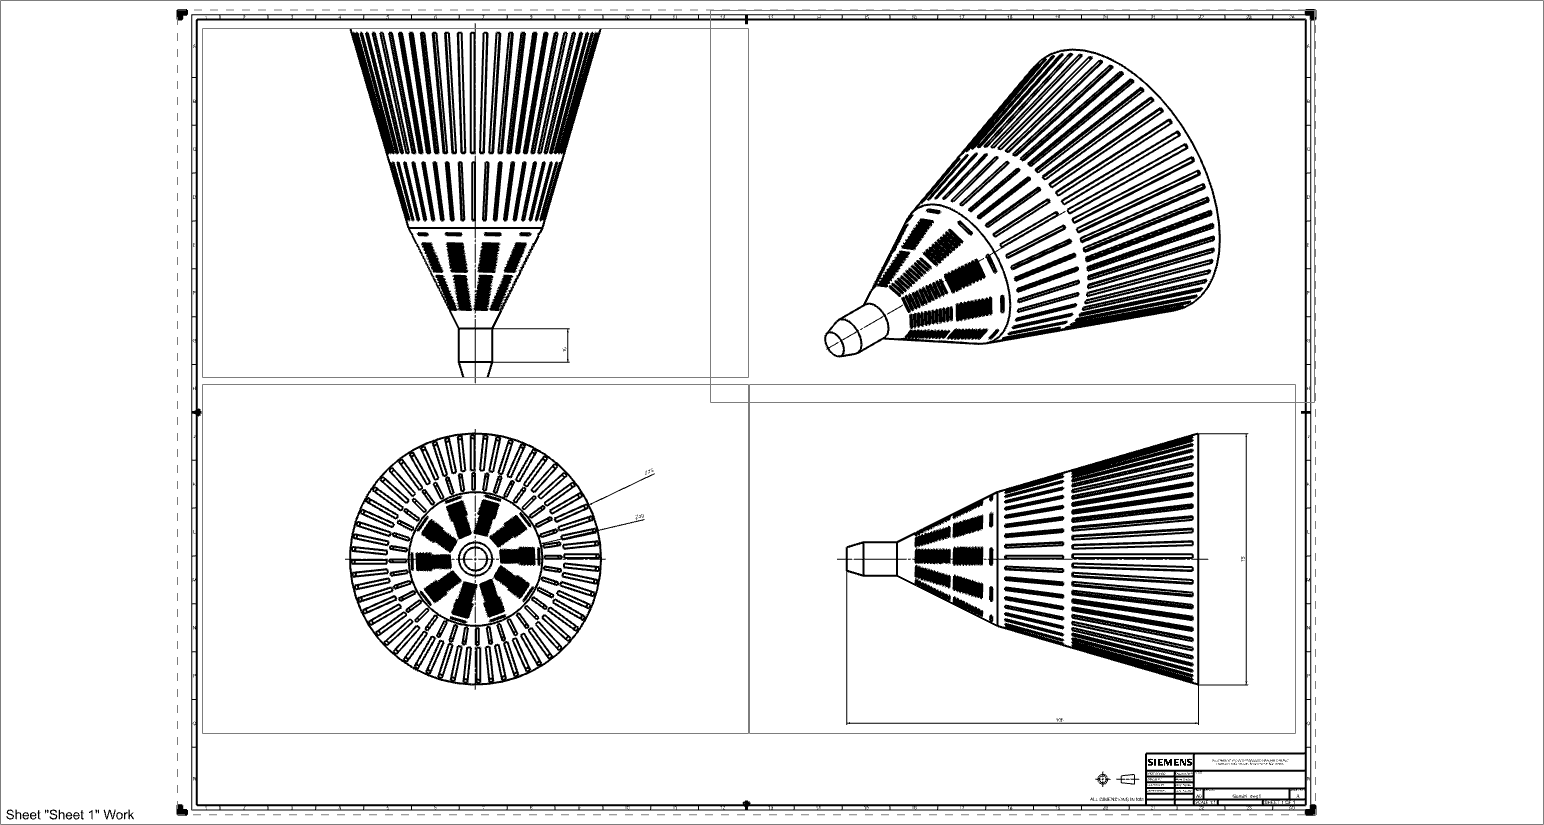
\includegraphics[width=\textwidth]{Woodson_3_View.png}
\end{figure}
\end{frame}

	\begin{frame}{DeVince: Beauty Shot}
\begin{figure}
	\centering
	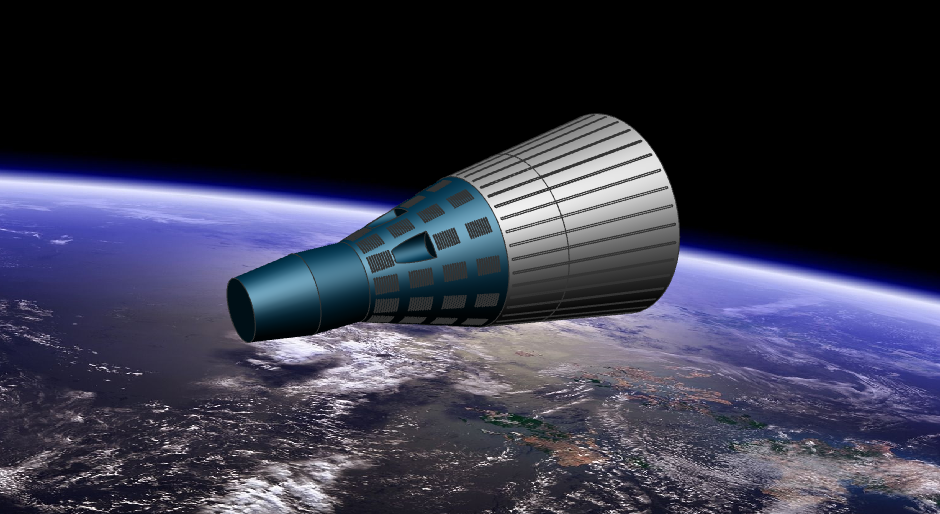
\includegraphics[width=\textwidth]{DeVince_Beauty.png}
\end{figure}
\end{frame}

\begin{frame}{DeVince: 3 View}
\begin{figure}
\centering
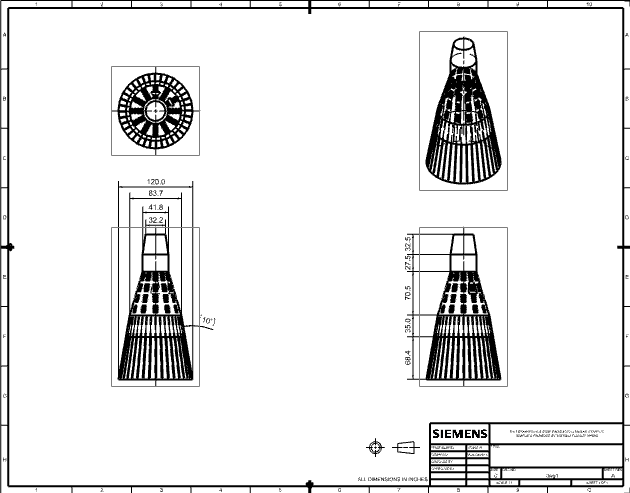
\includegraphics[width=\textwidth]{DeVince_3_View.png}
\end{figure}
\end{frame}

	\begin{frame}{Hanner: Beauty Shot}
\begin{figure}
	\centering
	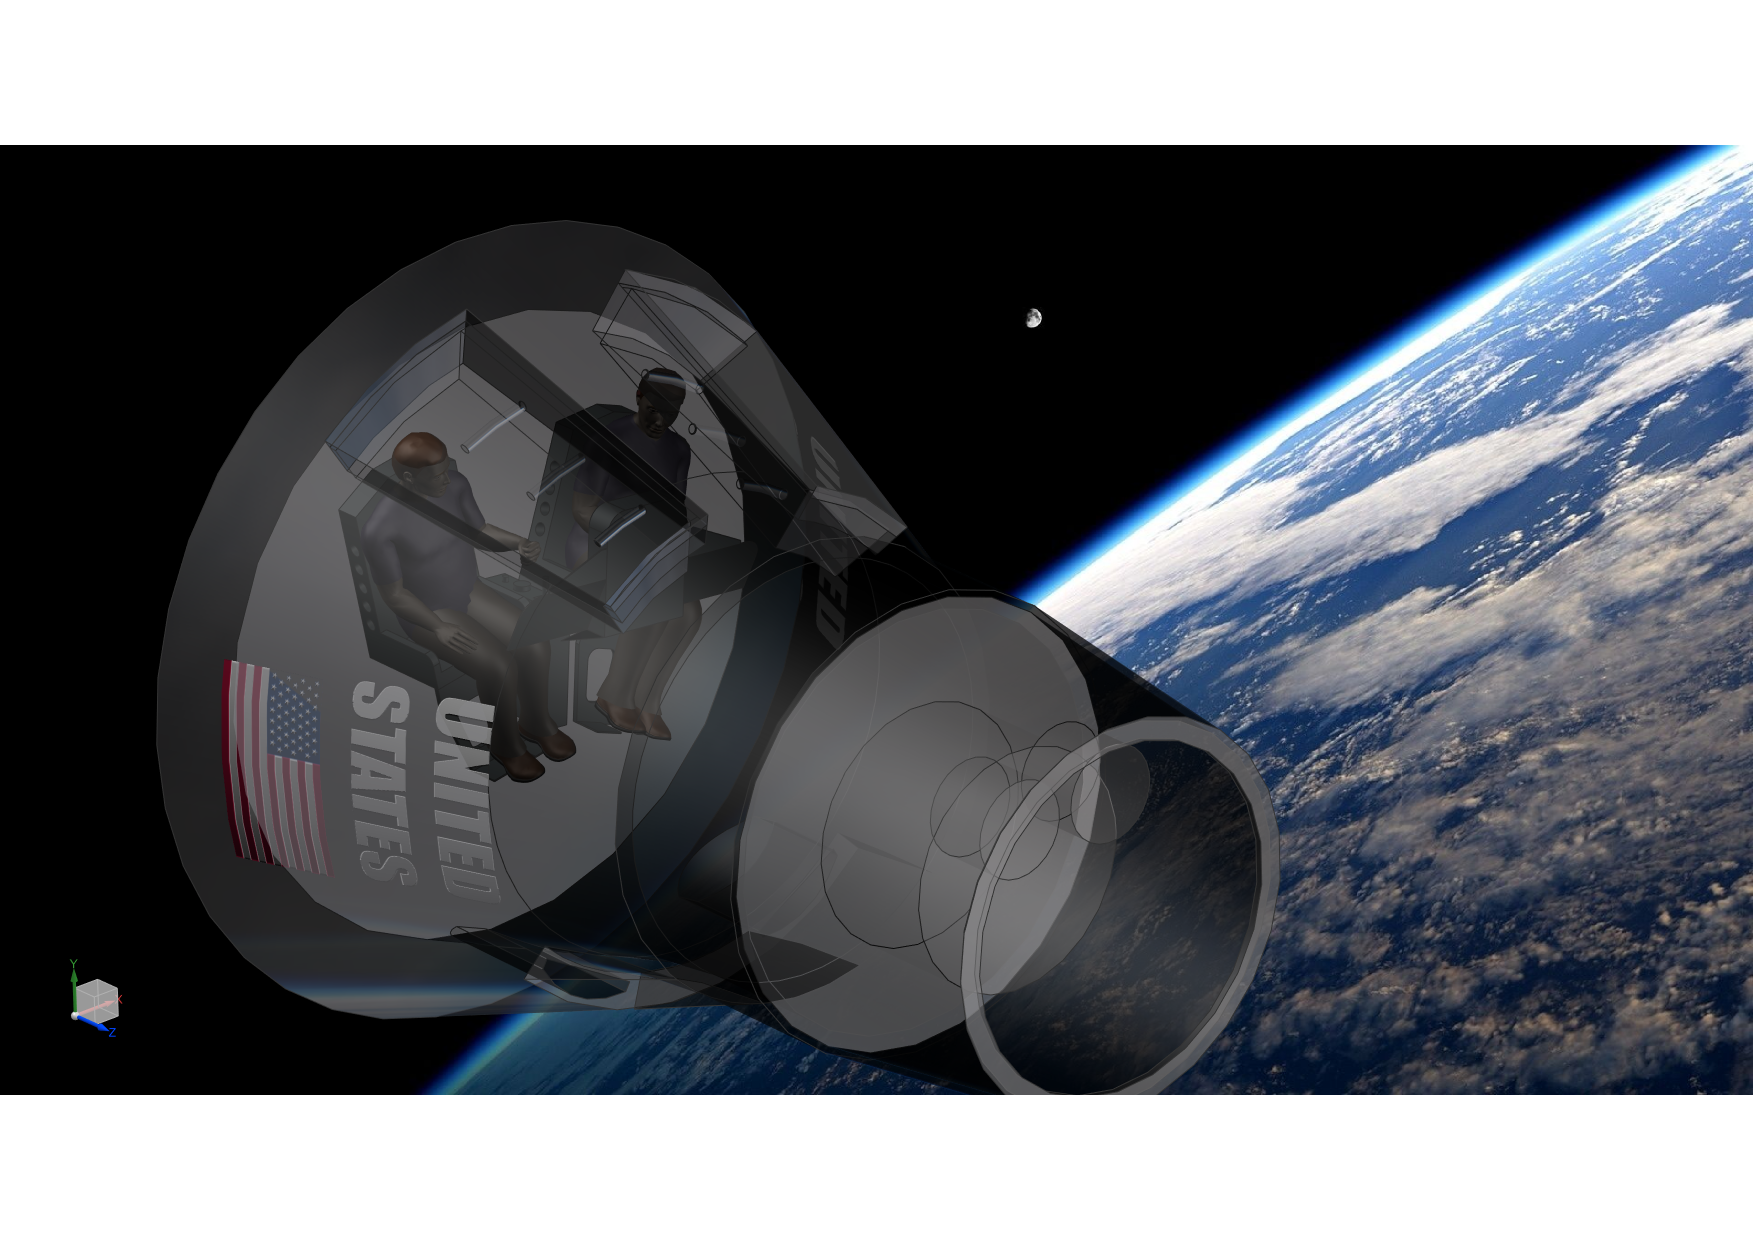
\includegraphics[width=\textwidth]{Hanner_Beauty.png}
\end{figure}
\end{frame}

\begin{frame}{Hanner: 3 View}
\begin{figure}
\centering
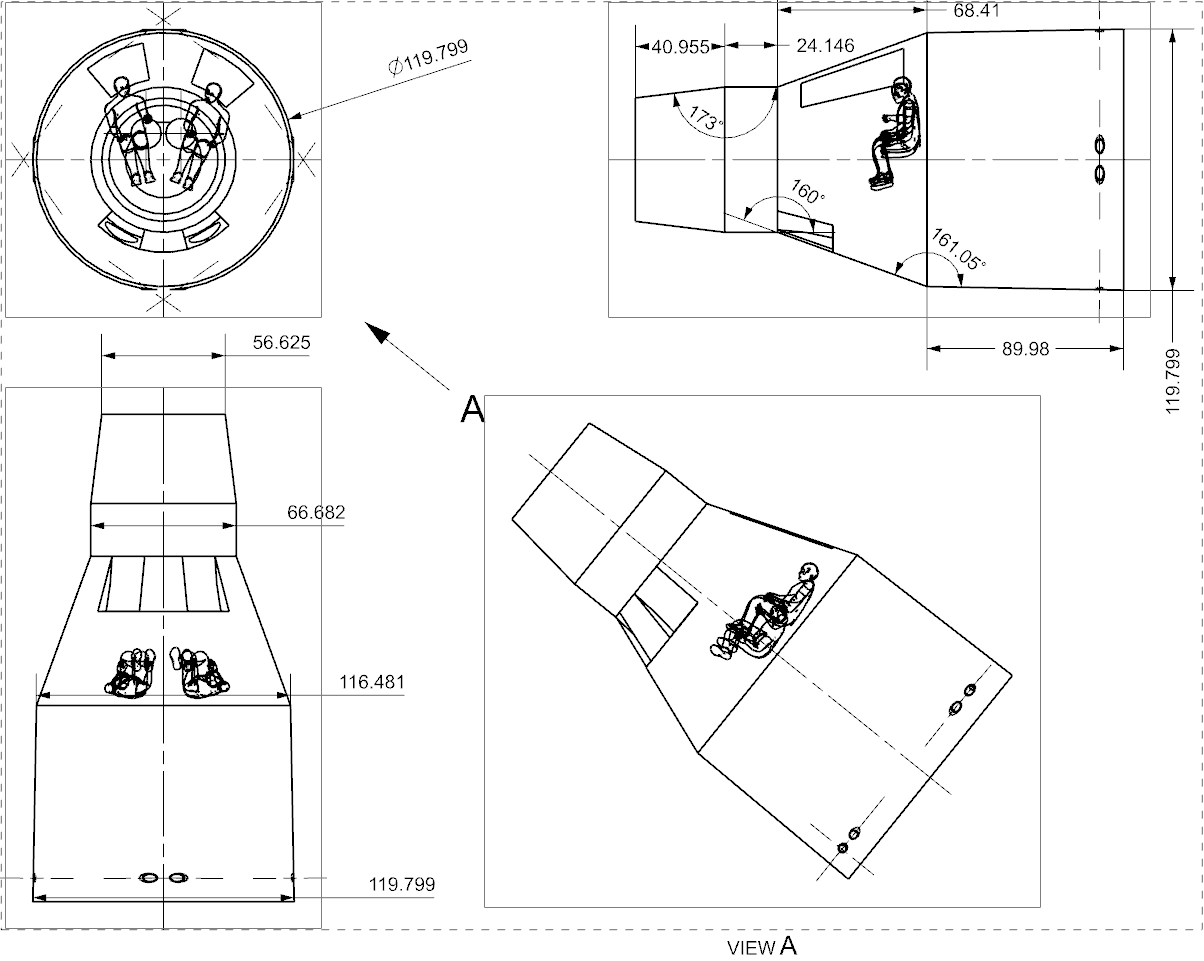
\includegraphics[width=\textwidth]{Hanner_3_View.png}
\end{figure}
\end{frame}

	\begin{frame}{Weinberg: Beauty Shot}
\begin{figure}
	\centering
	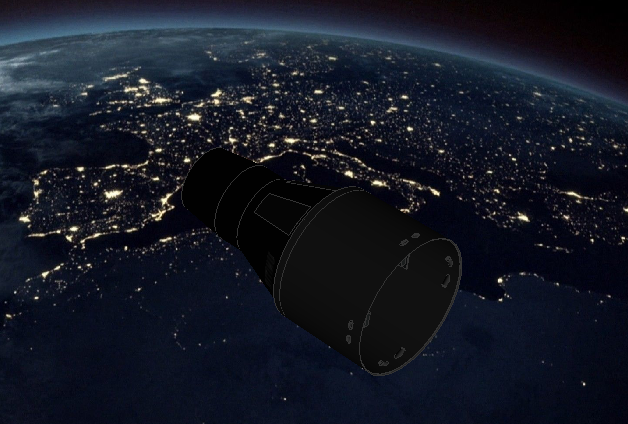
\includegraphics[width=\textwidth]{Weinberg_Beauty.png}
\end{figure}
\end{frame}

\begin{frame}{Weinberg: 3 View}
\begin{figure}
\centering
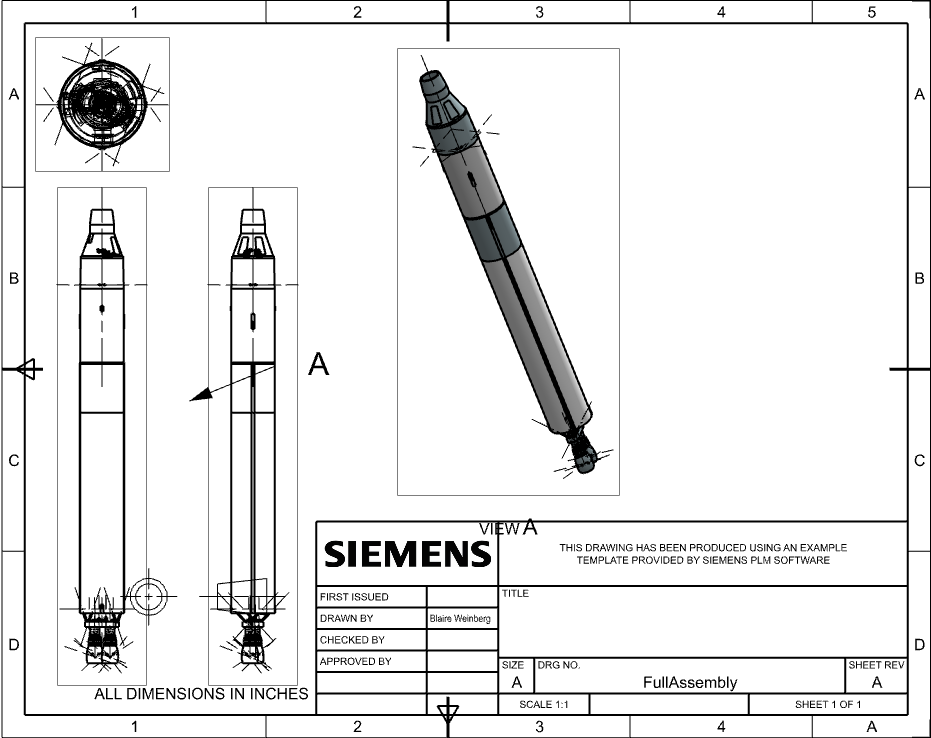
\includegraphics[width=\textwidth]{Weinberg_3_View.png}
\end{figure}
\end{frame}

	\begin{frame}{Chun: Beauty Shot}
\begin{figure}
	\centering
	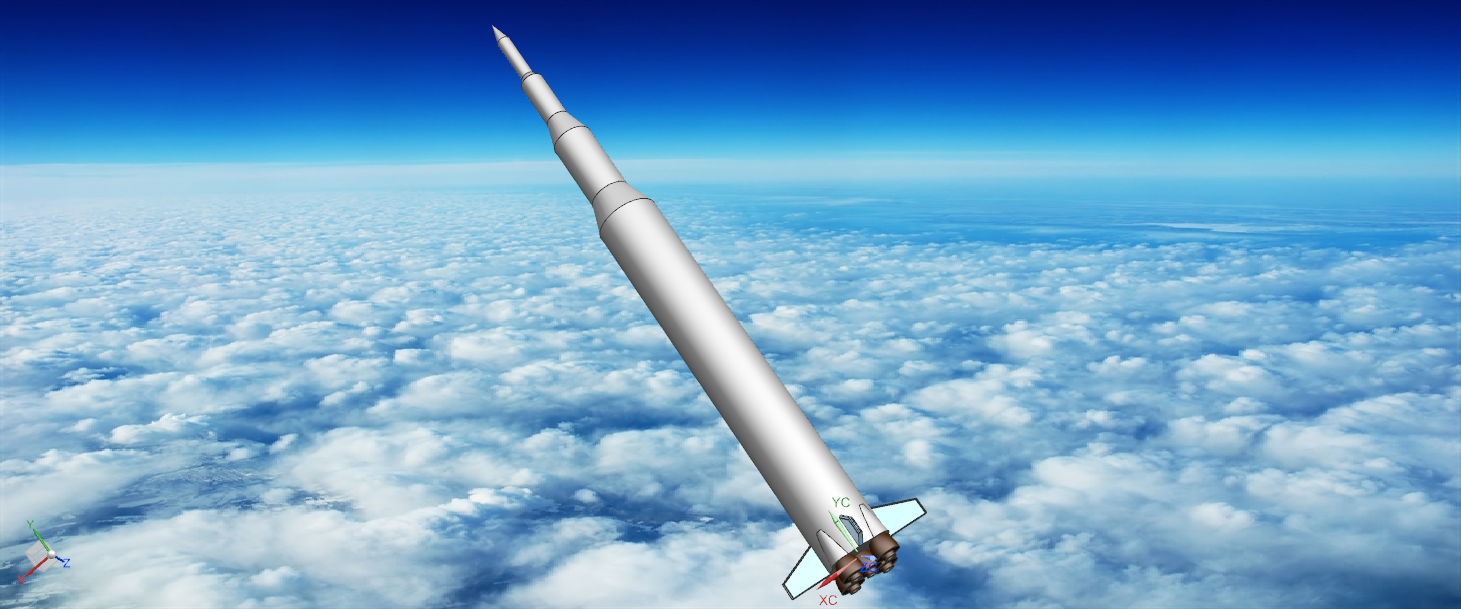
\includegraphics[width=\textwidth]{Chun_Beauty.png}
\end{figure}
\end{frame}

\begin{frame}{Chun: 3 View}
\begin{figure}
\centering
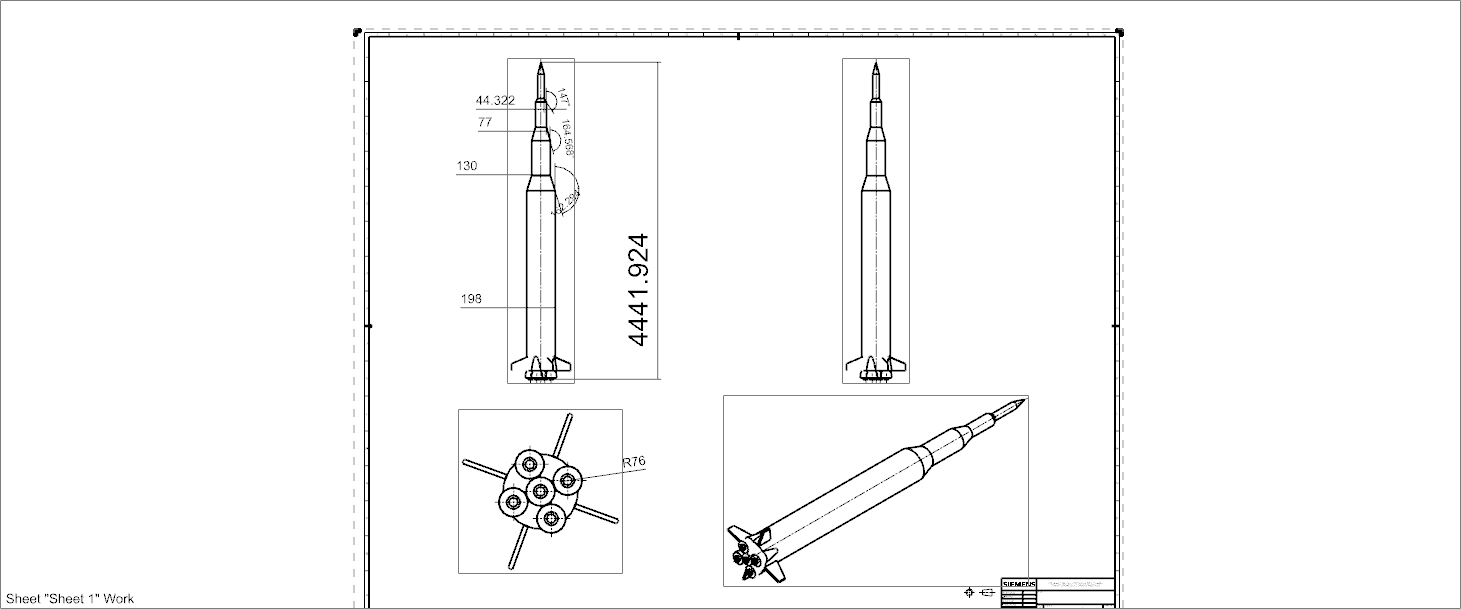
\includegraphics[width=\textwidth]{Chun_3_View.png}
\end{figure}
\end{frame}

\appendix
\begin{frame}{List of Parts}
\label{appx:A}
Due to the incompatibily issue between VLC and PC NX, there were a few components that could not be placed in the assembly. To show fair consideration to all members' work, we have attached a list of what parts individuals made. 
\begin{multicols}{2}

\begin{itemize}
	\item Ahmed Woodson
	\begin{itemize}
		\item Cryogenic O2 Tank
		\item Drinking Water Tank
		\item ECS Coolant Module
		\item Retrograde Rockets
		\item Retrograde Rocket Support
	\end{itemize}
	\item Mark DeVince
	\begin{itemize}
		\item Parachute System
		\item Orbit Attitude Control Thrusters
		\item Seats
		\item Center Console
		\item Communications Panel
		\item Instrumentation Panel
	\end{itemize}
	\item Charles Hanner
	\begin{itemize}
		\item First Stage Fairing 1
		\item First Stage Fairing 2
		\item Second Stage Fairing
		\item Upper Capsule
		\item Doors
		\item Lower Capsule 
	\end{itemize}
	\item Blaire Weinberg
	\begin{itemize}
		\item First Stage Engine
		\item Second Stage Engine
		\item First Stage Fuel Tank
		\item Second Stage Oxidizer Tank
		\item Second Stage Fuel Tank
	\end{itemize}
	\item Hyunsoo Chun
	\begin{itemize}
		\item Inertial Guidance Units
		\item Electrical Instrument
		\item Electrical Power System
		\item Reentry Controls System
	\end{itemize}
\end{itemize}
\end{multicols}
\end{frame}
\end{document}

